\documentclass{beamer}
\usetheme{Berkeley}

%%%
\usepackage{color}
\usepackage{xcolor}
\definecolor{keywordcolor}{rgb}{0.8,0.1,0.5}
\usepackage{listings}
\lstset{breaklines}%这条命令可以让LaTeX自动将长的代码行换行排版
\lstset{extendedchars=false}%这一条命令可以解决代码跨页时,章节标题,页眉等汉字不显示的问题
\lstset{language=C++, %用于设置语言为C++
	keywordstyle=\color{keywordcolor} \bfseries, %设置关键词
	identifierstyle=,
	basicstyle=\ttfamily, 
	commentstyle=\color{blue} \textit,
	stringstyle=\ttfamily, 
	showstringspaces=false,
	%frame=shadowbox, %边框
	captionpos=b
}
%%%
\usepackage{CJK}
\hypersetup{CJKbookmarks=true} %解决section不能使用中文的问题

\begin{document} %申明文档的开始
\begin{CJK}{UTF8}{gbsn}     %CJK:支持中文

	\title{Qt画线程序优化}
	\author{胡庆海}
	\date{}

    \begin{frame} %beamer里重要的概念,每个frame定义一张page
        \titlepage    % maketitle
    \end{frame}


    \begin{frame}
        \frametitle{主要内容}
        \tableofcontents
    \end{frame}

	\section{背景介绍}
	\begin{frame}[fragile]
        \frametitle{背景介绍}
		\framesubtitle{Qt画线程序代码}  

       	%\pause
        %Qt画线程序代码
		%\pause
		\begin{lstlisting}
		int main(int argc, char *argv[])
		{
			int i;
		   	return 0;
		}
		\end{lstlisting}

	\end{frame}

    \begin{frame}
        \frametitle{背景介绍}
        \pause
        相关定义....
        \begin{definition}
            definition定义 1...
        \end{definition}
    \end{frame}

	\section{热点分析}
    \begin{frame}
        \frametitle{热点分析}\pause
        \begin{itemize}
         \item beamer introd tion \pause
         \item beamer details \pause
         \item beamer conclusions
        \end{itemize}
    \end{frame}

	\section{优化方法}
    \begin{frame}
        \frametitle{优化方法}\pause
        \begin{itemize}
         \item beamer introd tion \pause
         \item beamer details \pause
         \item beamer conclusions
        \end{itemize}
    \end{frame}

	\section{效果分析}
    \begin{frame}
        \frametitle{效果分析}\pause
		\begin{figure}[!htbp]
			\centering
			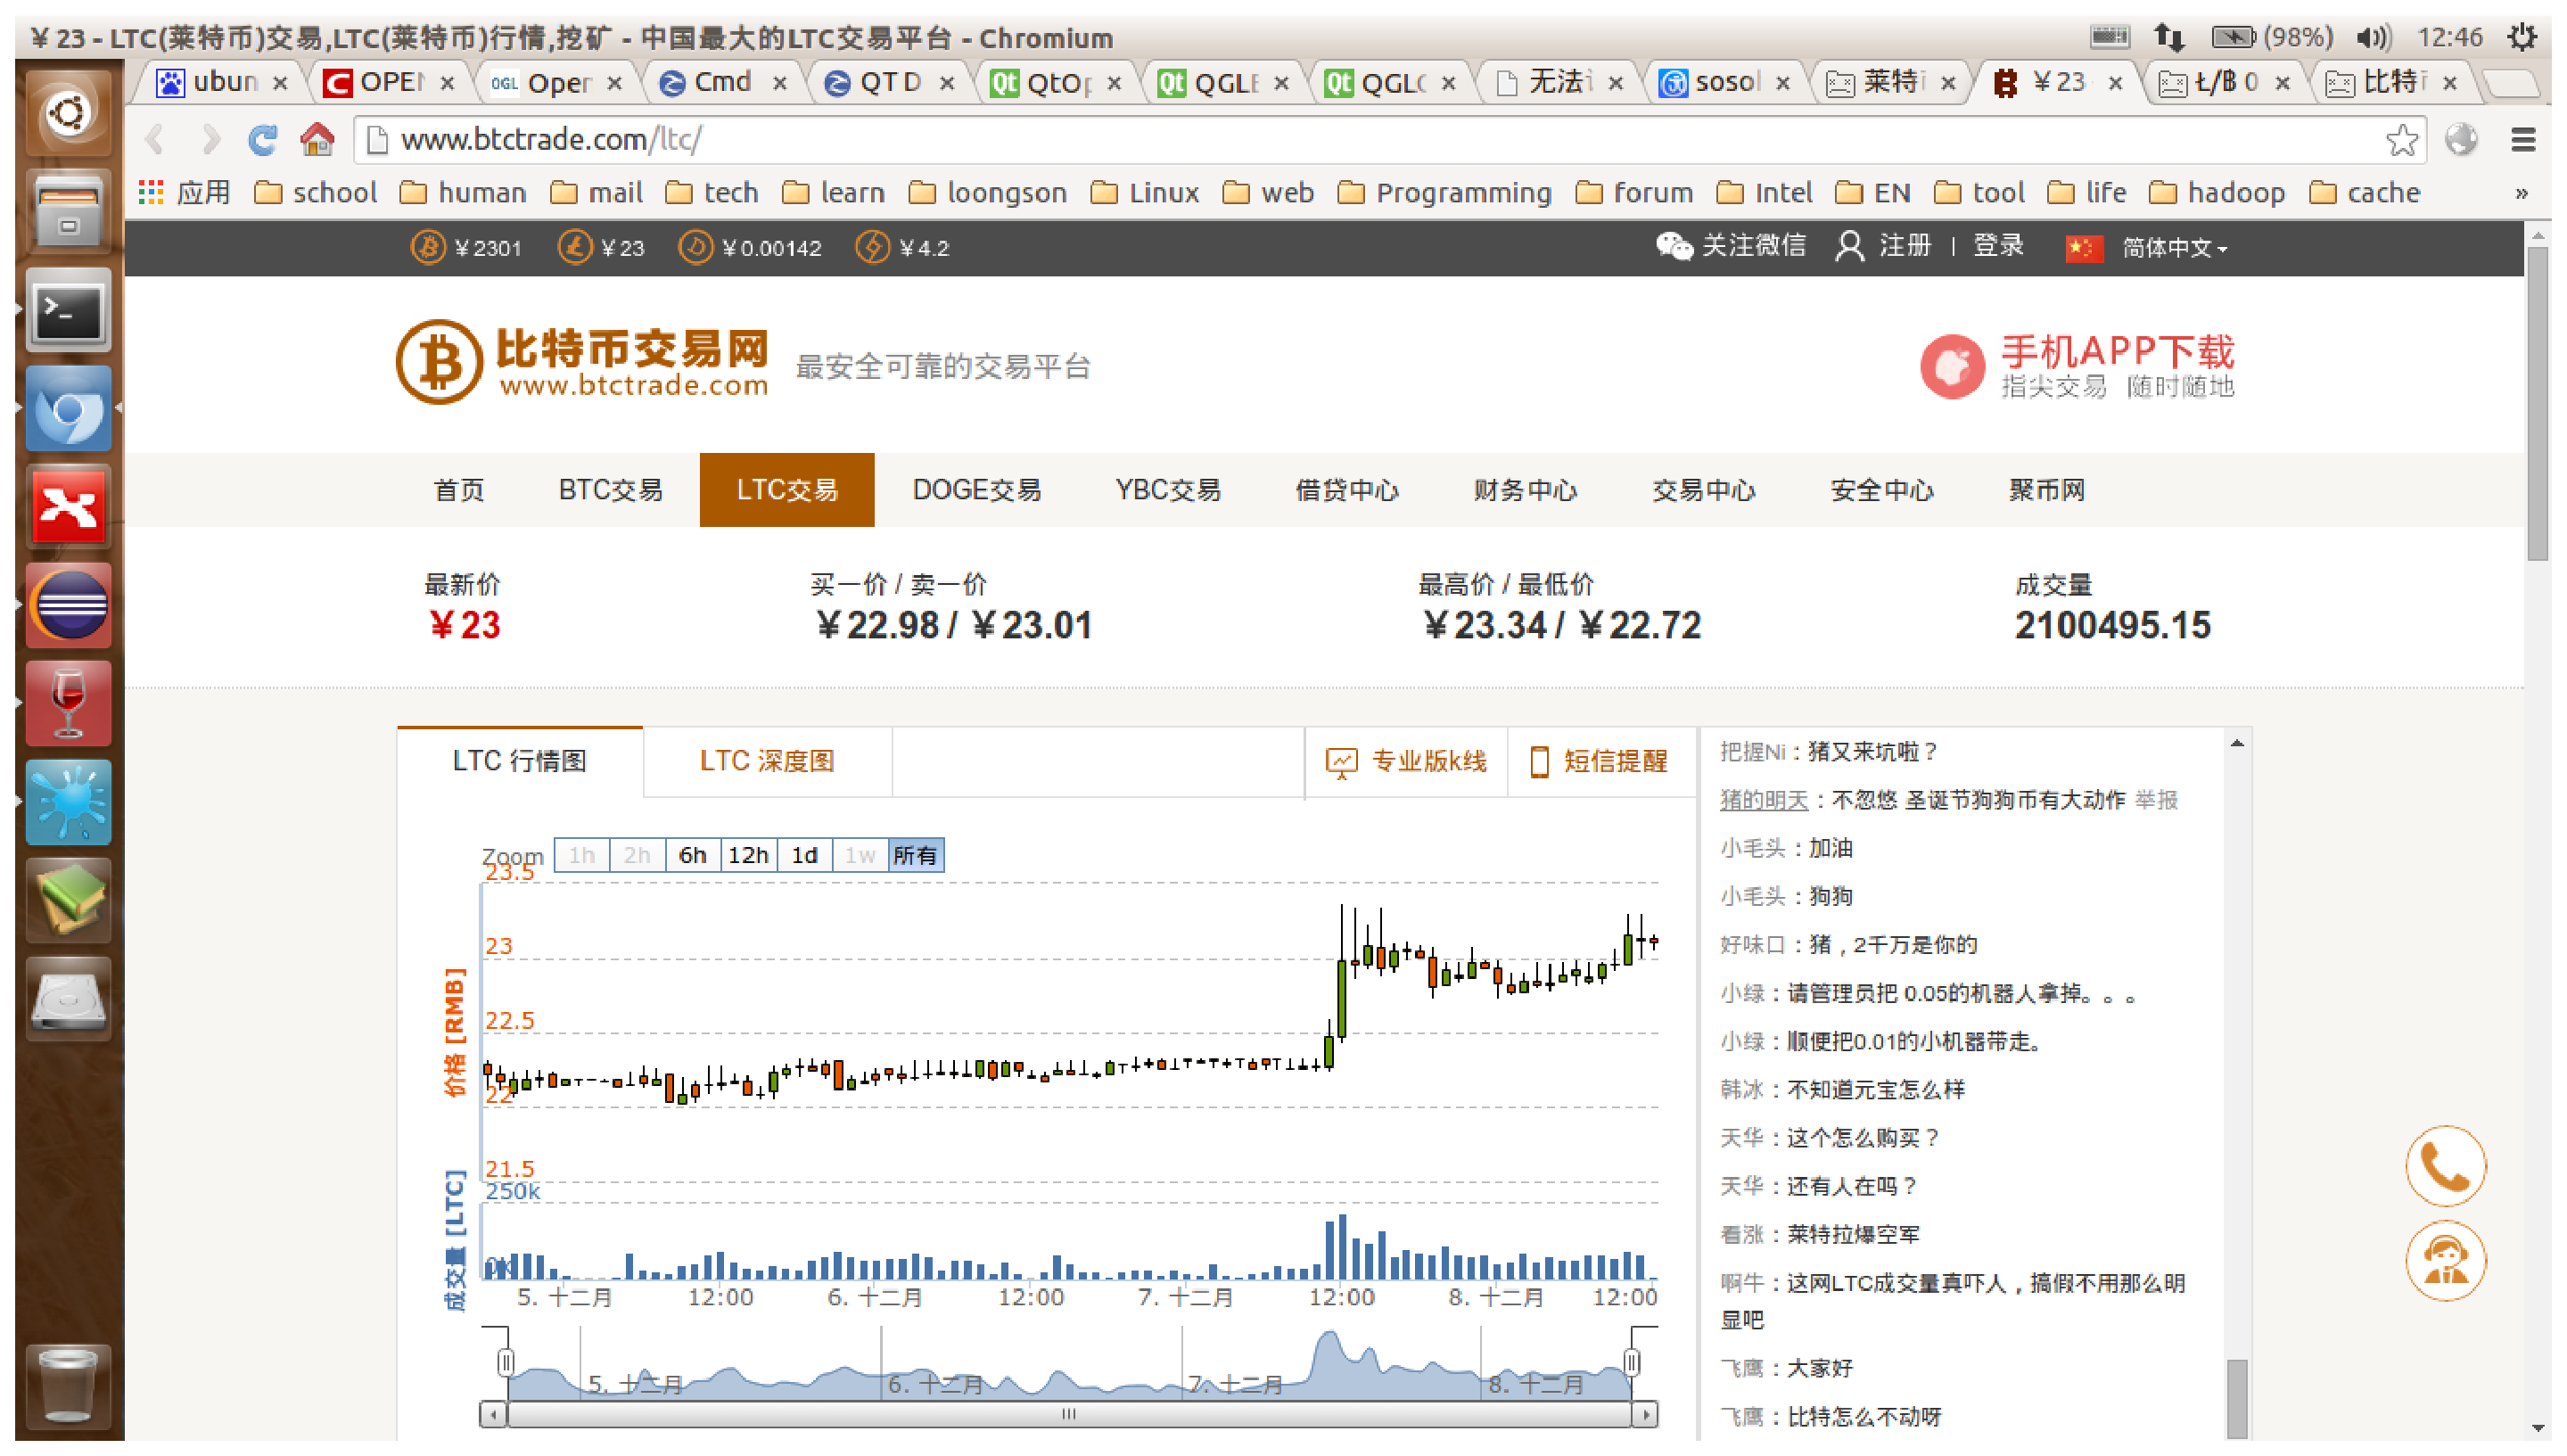
\includegraphics[width=10.00cm,height=7.10cm]{test.eps}
			\caption{一个图}
		\end{figure}
    \end{frame}

	\begin{frame}
		\frametitle{定理}
		\begin{lemma}[1]
		这是一个定理,引理类似。
		\end{lemma}
		\pause                       % 这里会暂停一下,pagedown会接着出现下面的式子
		\begin{displaymath}             %这个不用解释了吧
		1+1=2
		\end{displaymath}
		\begin{equation}
		1+1=2
		\end{equation}
	\end{frame}

	\begin{frame}\frametitle{插个表}
	一个表.
	 \begin{table}
	  \centering \addtolength{\tabcolsep}{1mm}
	 \begin{tabular}{ccccccccc}
	   \hline
	        & 1 & 2 & 3 & 4 & 5 & 6 & 7 & 8 \\
	   \hline
	    1 &         &       &          &       &       &       &       &  \\
	    2 & $c$     &       &          &       &       &       &       &  \\
	    3 & $c$     & $c $  &          &       &       &       &       &  \\
	    4 & $a$     & $a,c$ & $a $     &       &       &       &       &  \\
		5 & $a,b,c$ & $a,b$ & $a,b,c$  & $b,c$ &       &       &       &  \\
   		6 & $a,c$   & $a,c$ & $a,c$    & $c $  & $b,c$ &       &       &  \\
   		7 & $a,b,c$ & $a,b$ & $a,b,c$  & $b,c$ &       & $b,c$ &       &  \\
   		8 & $a,c$   & $a,c$ & $a,c$    & $c$   & $b,c$ &       & $b,c$ &  \\
   		\hline
		\end{tabular}\label{dismatrix}
		\end{table}
		\end{frame}

	\section{参考文献}
	\begin{frame}\frametitle{参考文献}
		[1] A\newline
		[2] B
	\end{frame}


	\begin{frame}\frametitle{致谢}
		Thanks
	\end{frame}


\end{CJK}
\end{document}
